\documentclass[11pt]{cernrep}
\usepackage{graphicx,epsfig}
\bibliographystyle{lesHouches}
\begin{document}

\setlength\parindent{0pt}

\title{Recasting activities at LH2017}

\author{L. Perrozzi$^1$, Fabio Maltoni, Sabine Kraml, Gabriel Facini, David Grellscheid, Sezen Sekmen, Johnatan Butterworth, Nishita Desai, Andy Buckley, Benjamin Fuks, Eric Conte, Peter Richardson, Olivier Mattelaer, Pasquale Musella, Alexandra Oliveira Carvalho, Ursula Laa, Kristin Lohwasser, Thrynova, Efe Yazgan, Philippe Gras, Sylvain}
\institute{
$^1$IPA at ETH Zurich, Switzerland
\\
$^2$...
}

\maketitle

\begin{abstract}
Recasting activities at Les Houches 2017.
\end{abstract}

\section{INTRODUCTION}

Searches for new physics constitute a basic ingredient of the LHC physics program.
Their variety and large number pose severe challenges to both the experimental and theory communities.
In fact, hundreds of searches are performed by different collaborations, a wide variety of final states is used, 
new ideas on how to probe new models and non-trivial signatures and improve the sensitivity of existing searches constantly emerge. 
The ultimate goal of this effort is to discover new physics if such
exists within the range of the LHC, and to test the widest possible range of hypothetical new physics models.

A typical analysis defines quantities that aid in classifying the event as signal or background: for example
the properties of analysis objects such as jets, electrons, muons, etc., or global event variables
such as object multiplicities, transverse momenta, transverse masses, etc.
An analysis can be very complex and feature many intricate definitions of object and event
variables, some of which cannot be expressed in closed algebraic form and must be defined
algorithmically. This complexity renders the task of visualizing, understanding, developing and
interpreting analyses increasingly challenging.  

One obvious way to cope with the complexity is to devise ways to enforce absolute clarity in the description of analyses.
A discussion was started in the Les Houches PhysTeV workshop in 2011, and continued
thereafter within a wider group of LHC physicists, in order to determine what information is
crucial for describing an analysis. The outcome of this discussion was reported in the 
\"Recommendations for Presentation of LHC Results\" [524,525], and has been embraced by many LHC physicists.

The current practice in our community is to write an analysis in non-public computer codes, 
which often rely on event objects specific to the experimental collaboration in question,
and then make public a description of the analysis via journal publications or other documents.

These efforts, which merit our great appreciation, 
have significantly increased the scientific value of many important experimental results. 

There is significant precedent for the effectiveness of such community standards. Several
accords have been established to standardize the communication of physics modeling information, 
notably the Les Houches Event Accord (LHE) [529, 530] and the SUSY Les Houches Accord (SLHA) [190, 531].
These, respectively, standardize the description of hard-process
particles in simulated collision events, and the details of all the parameters that define a BSM model point.  
Both accords are widely used in high-energy physics and have greatly helped to
simplify and make more efficient the communication between physicists.
In this report, we underscore the need for a standardized format — an “analysis description
accord” — capable of describing the contents of an analysis in an unambiguous way, which can
be fully exploited by the whole particle physics community.  The accord must be capable of
describing all object and event selections, as well as quantities such as efficiencies, analytic and
algorithmic observables, and advanced multivariate selections.
In the Les Houches PhysTeV workshop in 2015, a dedicated discussion has been initiated 
on how such an accord can be realized. 
The important motivations and use-cases for a standard analysis description accord were envisaged as:
\begin{itemize}
  \item Analysis preservation
  \item Analysis design
  \item Analysis review and communication
  \item Interpretation studies and analysis reimplementation
  \item Easier comparison of analyses
\end{itemize}
In addition, there are several desirable features which would further improve the utility
of the accord, which, however, may be nontrivial to simultaneously fulfill.  Therefore, here
we list all the desirable features, leaving it to the community discussion (and to individual
prototypes) to decide which of these desiderata should inform an eventual accord. We start by
listing the features we believe essential to the success of such an accord.

BASIC REQUIREMENTS:
\begin{itemize}
  \item Public availability
  \item Completeness
  \item Longevity
  \item Correctness and validatability
\end{itemize}
DESIRABLE FEATURES:
\begin{itemize}
  \item Human readability and writeability
  \item Self-contained
  \item Language independence
  \item Framework independence
  \item Support for combination of analyses
\end{itemize}

Several discussions and progresses have been made, but the proposal is not yet final and has not been widely adopted yet.

% In the following sections we shall detail the use cases
% and design requirements of such an accord, and the general pros and cons of several approaches.
The scope of this report, therefore, is to document the advancements obtained so far
on the recasting activities and attempt a first benchmark to compare different tools
to reproduce several ATLAS and CMS analyses' results.

\section{General Activities}

\begin{itemize}
  \item Feasibility study of the implementation/portability of complicated MVA techniques (BDT, NN,…) into the analyses
  \item Improvement of results and recastability: how to provide correlations signal systematics, possibility of providing a few key observables unfolded.
  \item Comparison of between DELPHES results and simple object smearing.
  \item Trying out the use of particle-level measurements to constrain model models
\end{itemize}

\section{Formats}
Object efficiency tables : which format (HEPDATA?)

\section{Benchmarking/Comparisons}

\begin{itemize}
  \item Implementation of analyses of increasing complexity in the Analysis Description Format (LHADA Proposal) and in (BSM) Rivet and their comparison.
  \item Choose an analysis of ATLAS or CMS which has cutflow and detector effects provided in some form, and possibly is already been implemented in the recasting codes CheckMate/MadAnalysis/Rivet/ATOM.
  \item Implement the same analysis in LHADA and then use the dedicated parsers to provide the analysis for the recasting codes.
  \item Reproduce the NP interpretation of the original paper (=validation implementation).
  \item Recast the analysis for an other new physics model and compare the results.
  \item Go to point one and choose a more complicated analysis…
\end{itemize}
it would be interesting to see how Delphes performance looks without analysis-specific cards, since a lot of people (outside the “big” recasting groups) are using it that way.

\section{How to validate the analyses}
\begin{figure}
\begin{center}
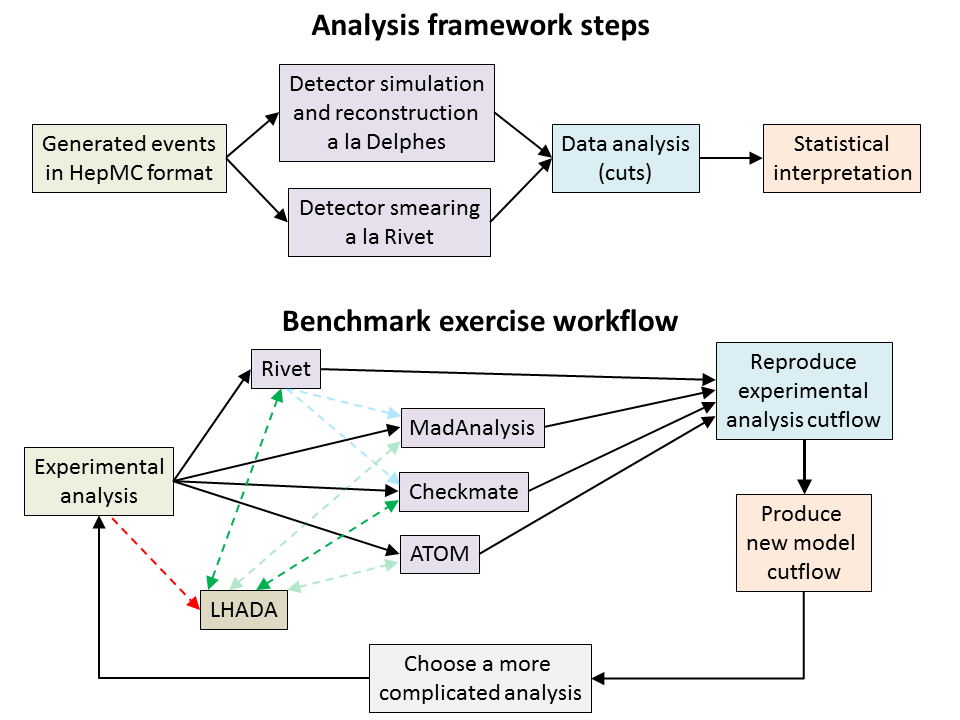
\includegraphics[width=0.5\textwidth]{figures/lhada_benchmarking_excersise.png}
 \caption{Search reach for the $\mu \gamma {\not\!\!E}_{T}$ signal
(as defined in the
   text) for
   300 fb$^{-1}$ integrated luminosity  at the LHC.
}
\label{search}
\end{center}
\end{figure}


\section{The analysis frameworks and tools}
In this section we describe the analysis frameworks and tools used for the comparison and benchmarking
\subsection{ATOM}
Brief description of ATOM
\subsection{CheckMate}
Brief description of CheckMate
\subsection{MadAnalysis}
Brief description of MadAnalysis
\subsection{Rivet}
Brief description of Rivet
\subsection{Generic Analysis Description Proposal}
Brief description of the Generic Analysis Description Proposal

\section{Analyses benchmarking, comparisons and results}

\subsection{arxiv:1605.03814 - Jets+MET - ATLAS - 13 TeV}
Brief description of the ATLAS analysis Jets+MET at 13 TeV (arxiv:1605.03814). 
Results are reported in table~\ref{tab:1605.03814}.

\begin{table*}[htbp]
\tiny
	\centering
		\begin{tabular}{ | l || l | l | l || l | l | l || l | }
\hline
% Rivet, MadAnalysis 5 and CheckMATE2 benchmarking results & \  & \  & \  & \  & \  & \  & \  & \  \\ \hline
% arxiv:1605.03814 - Jets+MET - ATLAS - 13 TeV & \  & \  & \  & \  & \  & \  & \  & \  \\ \hline
% Gluino mass 1600 - N1 mass 0 & \  & \  & \  & \  & \  & \  & \  & \  \\ \hline
% Rivet default (with efficiencies and smearing); MadAnalysis5 default; CheckMATE2 default & \  & \  & \  & \  & \  & \  & \  & \  \\ \hline
 % & \  & \  & \  & \  & \  & \  & \  & \  \\ \hline
                  &  \multicolumn{3}{c||}{\bf Rivet} & \multicolumn{3}{c||}{\bf MadAnalysis5} &   {\bf CheckMATE}   \\ \hline

Description       & \#evt & tot.eff & rel.eff & \#evt & tot.eff & rel.eff &   tot.eff   \\ \hline \hline
{\bf 2jl cut-flow}                  & 31250 & 1 & - & 31250 & 1 & - & \   \\ \hline
Pre-sel+MET+pT1   & 28592 & 0.91 & 0.91 & 28626 & 0.92 & 0.92 & \   \\ \hline
Njet              & 28592 & 0.91 & 1 & 28625 & 0.92 & 1 & \   \\ \hline
Dphi\_min(j,MET)   & 17297 & 0.55 & 0.6 & 17301 & 0.55 & 0.6 & \   \\ \hline
pT2               & 17067 & 0.55 & 0.99 & 17042 & 0.55 & 0.99 & \   \\ \hline
MET/sqrtHT        & 8900 & 0.28 & 0.52 & 8898 & 0.28 & 0.52 & \   \\ \hline
m\_eff(incl)       & 8896 & 0.28 & 1 & 8897 & 0.28 & 1 & \   \\ \hline
\hline
{\bf 2jm cut-flow} & 31250 & 1 & - & 32150 & 1 & - & 1  \\ \hline
Pre-sel+MET+pT1   & 28472 & 0.91 & 0.91 & 28478 & 0.91 & 0.91 & 0.91  \\ \hline
Njet              & 28472 & 0.91 & 1 & 28477 & 0.91 & 1 & 0.91  \\ \hline
Dphi\_min(j,MET)   & 22950 & 0.73 & 0.81 & 22889 & 0.73 & 0.8 & 0.73  \\ \hline
pT2               & 22950 & 0.73 & 1 & 22889 & 0.73 & 1 & 0.73  \\ \hline
MET/sqrtHT        & 10730 & 0.34 & 0.47 & 10710 & 0.34 & 0.47 & 0.33  \\ \hline
m\_eff(incl)       & 10630 & 0.34 & 0.99 & 10609 & 0.34 & 0.99 & 0.32  \\ \hline
\hline
{\bf 2jt cut-flow} & 31250 & 1 & - & 31250 & 1 & - & \   \\ \hline
Pre-sel+MET+pT1   & 28592 & 0.91 & 0.91 & 28626 & 0.92 & 0.92 & \   \\ \hline
Njet              & 28592 & 0.91 & 1 & 28625 & 0.92 & 1 & \   \\ \hline
Dphi\_min(j,MET)   & 17297 & 0.55 & 0.6 & 17301 & 0.55 & 0.6 & \   \\ \hline
pT2               & 17067 & 0.55 & 0.99 & 17042 & 0.55 & 0.99 & \   \\ \hline
MET/sqrtHT        & 5083 & 0.16 & 0.3 & 5098 & 0.16 & 0.3 & \   \\ \hline
Pass m\_eff(incl)  & 4861 & 0.16 & 0.96 & 4889 & 0.16 & 0.96 & \   \\ \hline
\hline
{\bf 4jt cut-flow} & 31250 & 1 & - & 31250 & 1 & - & 1  \\ \hline
Pre-sel+MET+pT1   & 28592 & 0.91 & 0.91 & 28626 & 0.92 & 0.92 & 0.91  \\ \hline
Njet              & 27322 & 0.87 & 0.96 & 27128 & 0.87 & 0.95 & 0.87  \\ \hline
Dphi\_min(j,MET)   & 18929 & 0.61 & 0.69 & 18829 & 0.6 & 0.69 & 0.6  \\ \hline
pT2               & 18715 & 0.6 & 0.99 & 18825 & 0.6 & 1 &     --       \\ \hline
pT4               & 16610 & 0.53 & 0.89 & 16430 & 0.53 & 0.87 & 0.52  \\ \hline
Aplanarity        & 11849 & 0.38 & 0.71 & 11395 & 0.36 & 0.69 & 0.36  \\ \hline
MET/m\_eff(Nj)     & 8334 & 0.27 & 0.7 & 7971 & 0.26 & 0.7 & 0.25  \\ \hline
m\_eff(incl)       & 7201 & 0.23 & 0.86 & 6972 & 0.22 & 0.87 & 0.21  \\ \hline
\hline
{\bf 5j cut-flow} & 31250 & 1 & - & 31250 & 1 & - & 1 \\ \hline
Pre-sel+MET+pT1   & 28592 & 0.91 & 0.91 & 28626 & 0.92 & 0.92 & 0.91 \\ \hline
Njet              & 21234 & 0.68 & 0.74 & 21185 & 0.68 & 0.74 & 0.68 \\ \hline
Dphi\_min(j,MET)   & 14294 & 0.46 & 0.67 & 14292 & 0.46 & 0.67 & 0.45 \\ \hline
pT2               & 14146 & 0.45 & 0.99 & 14289 & 0.46 & 1 &    --       \\ \hline
pT4               & 13229 & 0.42 & 0.94 & 13228 & 0.42 & 0.93 & 0.42 \\ \hline
Aplanarity        & 9836 & 0.31 & 0.74 & 9576 & 0.31 & 0.72 & 0.3 \\ \hline
MET/m\_eff(Nj)     & 4643 & 0.15 & 0.47 & 4506 & 0.14 & 0.47 & 0.13 \\ \hline
m\_eff(incl)       & 4620 & 0.15 & 1 & 4476 & 0.14 & 0.99 & 0.13 \\ \hline
\hline
{\bf 6jm cut-flow} & 31250 & 1 & - & 31250 & 1 & - & 1  \\ \hline
Pre-sel+MET+pT1   & 28592 & 0.91 & 0.91 & 28626 & 0.92 & 0.92 & 0.91  \\ \hline
Njet              & 13235 & 0.42 & 0.46 & 13236 & 0.42 & 0.46 & 0.41  \\ \hline
Dphi\_min(j,MET)   & 8520 & 0.27 & 0.64 & 8553 & 0.27 & 0.65 & 0.26  \\ \hline
pT2               & 8436 & 0.27 & 0.99 & 8551 & 0.27 & 1 &    --        \\ \hline
pT4               & 8135 & 0.26 & 0.96 & 8217 & 0.26 & 0.96 & 0.25  \\ \hline
Aplanarity        & 6365 & 0.2 & 0.78 & 6307 & 0.2 & 0.77 & 0.19  \\ \hline
MET/m\_eff(Nj)     & 2675 & 0.09 & 0.42 & 2665 & 0.09 & 0.42 & 0.08  \\ \hline
m\_eff(incl)       & 2670 & 0.09 & 1 & 2656 & 0.08 & 1 & 0.08  \\ \hline
\hline
{\bf 6jt cut-flow} & 31250 & 1 & - & 31250 & 1 & - & \   \\ \hline
Pre-sel+MET+pT1   & 28592 & 0.91 & 0.91 & 28626 & 0.92 & 0.92 & \   \\ \hline
Njet              & 13235 & 0.42 & 0.46 & 13236 & 0.42 & 0.46 & \   \\ \hline
Dphi\_min(j,MET)   & 8520 & 0.27 & 0.64 & 8553 & 0.27 & 0.65 & \   \\ \hline
pT2               & 8436 & 0.27 & 0.99 & 8551 & 0.27 & 1 & \   \\ \hline
pT4               & 8135 & 0.26 & 0.96 & 8217 & 0.26 & 0.96 & \   \\ \hline
Aplanarity        & 6365 & 0.2 & 0.78 & 6307 & 0.2 & 0.77 & \   \\ \hline
MET/m\_eff(Nj)     & 3900 & 0.12 & 0.61 & 3839 & 0.12 & 0.61 & \   \\ \hline
m\_eff(incl)       & 3715 & 0.12 & 0.95 & 3672 & 0.12 & 0.96 & \   \\ \hline
			
		\end{tabular}
	\caption{1605.03814 cut flow}
	\label{tab:1605.03814}
\end{table*}

\subsection{arxiv:1704.03848 - Monophoton - ATLAS - 13 TeV}
Brief description of the ATLAS analysis Monophoton at 13 TeV (arxiv:1704.03848).

\subsection{CMS-SUS-16-039 - 3 leptons + MET - CMS - 13 TeV}
Brief description of the CMS analysis 3 leptons + MET at 13 TeV (CMS-SUS-16-039).

\subsection{arxiv:1706.04402 - 1 lepton + MET + Jets (>=1b) - CMS - 13 TeV} (topness variable?)
Brief description of the CMS analysis 1 lepton + MET + Jets ($>=1b$) (topness variable) at 13 TeV (arxiv:1706.04402).

\section*{CONCLUSIONS}
We are cool.

\section*{ACKNOWLEDGEMENTS}
We acknowledge the acknowledgements.

\bibliography{sample_bib}

\end{document}
